%! Author = Bartosz Walusiak, Krzysztof Zdulski, Monika Lewandowska
%! Date = 11/16/2019

% Preamble
\documentclass[a4paper, 12pt]{article}

\usepackage{float}
\usepackage[T1]{fontenc}
\usepackage{lmodern}
\usepackage[polish]{babel}
\usepackage[utf8]{inputenc}
\usepackage{polski}
\usepackage{hyperref}
\usepackage{karnaugh-map}
\usepackage{amsmath}
\usepackage{ulem}
\usepackage{bm}
\usepackage{graphicx}

\newcounter{implicant_counter}
\newcommand{\imp}[1]{
I\textsubscript{\arabic{implicant_counter}}
\label{imp:#1-\arabic{implicant_counter}}
\stepcounter{implicant_counter}
}

\begin{document}
    \title{Projekt nr 1 POTEC}
    \author{Monika Lewandowska, Bartosz Walusiak, Krzysztof Zdulski}
    \date{\today}
    \maketitle

    \tableofcontents

    \newpage
    \section{Wstęp}\label{sec:intro}
    \subsection{Cel projektu}\label{subsec:intro-goal}
Projekt ma na celu analizę i realizację siedmiosegmentowego układu obwodu dekodera, którego aktywnym sygnałem jest $0$.
Wyświetlacze siedmiosegmentowe są tymi najczęściej stosowanymi do
wyświetlenia liczb (w celu uzyskania odczytu dziesiętnego).

\subsection{Realizacja projektu}\label{subsec:intro-how}
Realizacja układu dekodera została podzielona na 3 etapy:
\begin{enumerate}
    \item Zapisano tablicę prawdy dla każdego z segmentów - przedstawioną w Tablicy~\ref{tab:truth-table}.
    \item Wyznaczono minimalne postaci każdej z funkcji korzystając
          z metod minimalizacji tablic Karnaugha oraz Espresso.
    \item Zrealizowano dekoder przy użyciu oprogramowania Logisim, mając na uwadze fakt,
          iż aktywnym sygnałem w tym programie jest $1$.
\end{enumerate}

\begin{table}[H]
    \centering
    \begin{tabular}{|c||c|c|c|c||c|c|c|c|c|c|c|}
        \hline
        Cyfra & $x_3$ & $x_2$ & $x_1$ & $x_0$ & $f_a$ & $f_b$ & $f_c$ & $f_d$ & $f_e$ & $f_f$ & $f_g$ \\ \hline
        \hline
        0     & 0     & 0     & 0     & 0     & 0     & 0     & 0     & 0     & 0     & 0     & 1     \\ \hline
        1     & 0     & 0     & 0     & 1     & 1     & 0     & 0     & 1     & 1     & 1     & 1     \\ \hline
        2     & 0     & 0     & 1     & 0     & 0     & 0     & 1     & 0     & 0     & 1     & 0     \\ \hline
        3     & 0     & 0     & 1     & 1     & 0     & 0     & 0     & 0     & 1     & 1     & 0     \\ \hline
        4     & 0     & 1     & 0     & 0     & 1     & 0     & 0     & 1     & 1     & 0     & 0     \\ \hline
        5     & 0     & 1     & 0     & 1     & 0     & 1     & 0     & 0     & 1     & 0     & 0     \\ \hline
        6     & 0     & 1     & 1     & 0     & 0     & 1     & 0     & 0     & 0     & 0     & 0     \\ \hline
        7     & 0     & 1     & 1     & 1     & 0     & 0     & 0     & 1     & 1     & 1     & 1     \\ \hline
        8     & 1     & 0     & 0     & 0     & 0     & 0     & 0     & 0     & 0     & 0     & 0     \\ \hline
        9     & 1     & 0     & 0     & 1     & 0     & 0     & 0     & 0     & 1     & 0     & 0     \\ \hline
    \end{tabular}
    \caption{Tablica prawdy dekodera}
    \label{tab:truth-table}
\end{table}

    \newpage
    \section{Zadanie 1 - Minimalizacja funkcji boolowskiej za pomocą tablic Karnaugha dla mintermów}\label{sec:task-1}
    \subsection{Funkcja g}\label{subsec:fun-g}
    Funkcja $f_g$ zapisana w postaci mintermów wygląda następująco.
\[f_g(x_3, x_2, x_1, x_0) = \sum (0, 1, 7, (10, 11, 12, 13, 14, 15))\]
\begin{figure}[H]
    \centering
    \begin{karnaugh-map}[4][4][1][$x_{1}x_0$][$x_{3}x_2$]
        \minterms{0, 1, 7}
        \maxterms{2, 3, 4, 5, 6, 8, 9}
        \indeterminants{10, 11, 12, 13, 14, 15}
        \implicant{0}{1}
        \implicant{7}{15}
    \end{karnaugh-map}
    \caption{Tablica dla funkcji \textrm{g}}
    \label{fig:fg}
\end{figure}
Minimalizację funkcji $f_g(x_3, x_2, x_1, x_0)$ za pomocą tablicy Karnaugha przedstawiono na Rys.~\ref{fig:fg}.
Znaleziono 2 implikanty proste, z których wszystkie są niezbędne (\textrm{EIP}).
\begin{equation}
    \label{eq:fg}
    f_g(x_3, x_2, x_1, x_0) = x_3'x_2'x_1'+x_{2}x_{1}x_0
\end{equation}
Równanie~\ref{eq:fg} jest zminimalizowanym równaniem funkcji  $f_g$.


    \newpage
    \section{Zadanie 2 - Minimalizacja funkcji boolowskiej za pomocą tablic Karnaugha dla maxtermów}\label{sec:task-2}
    \subsection{Funkcja a}\label{subsec:fun-a}
    Funkcja $f_a$ zapisana w postaci maxtermów wygląda następująco.
\[f_a(x_3, x_2, x_1, x_0) = \prod (1, 4, (10, 11, 12, 13, 14, 15))\]
\begin{figure}[h]
    \centering
    \begin{karnaugh-map}[4][4][1][$x_1x_0$][$x_3x_2$]
        \minterms{0, 2, 3, 5, 6, 7, 8, 9}
        \maxterms{1, 4}
        \indeterminants{10, 11, 12, 13, 14, 15}
        \implicant{4}{12}
        \implicant{1}{1}
    \end{karnaugh-map}
    \caption{Tabela dla funkcji \textrm{a}}
    \label{fig:fa}
\end{figure}
Minimalizację funkcji $f_a(x_3, x_2, x_1, x_0)$ za pomocą tablicy Karnaugha przedstawiono na Rys.~\ref{fig:fa}.
Znaleziono 2 implikanty proste, z których wszystkie były niezbędne (\textrm{EIP}).
\begin{equation}
    \label{eq:fa}
    f_a(x_3, x_2, x_1, x_0) = (x_0 + x_1 + x_2')(x_0' + x_1 + x_2 + x_3)
\end{equation}
Równanie~\ref{eq:fa} jest zminimalizowanym równaniem funkcji  $f_a$.

    \newpage
    \subsection{Funkcja b}\label{subsec:fun-b}
    Funkcja $f_b$ zapisana w postaci maxtermów wygląda następująco.
\[f_b(x_3, x_2, x_1, x_0) = \prod (0, 1, 2, 3, 4, 7, 8, 9, (10, 11, 12, 13, 14, 15))\]
\begin{figure}[h]
    \centering
    \begin{karnaugh-map}[4][4][1][$x_{1}x_0$][$x_{3}x_2$]
        \minterms{5, 6}
        \maxterms{0, 1, 2, 3, 4, 7, 8, 9}
        \indeterminants{10, 11, 12, 13, 14, 15}
        \implicant{0}{2}
        \implicant{8}{10}
        \implicant{0}{8}
        \implicant{3}{11}
    \end{karnaugh-map}
    \caption{Tablica dla funkcji \textrm{b}}
    \label{fig:fb}
\end{figure}
Minimalizację funkcji $f_b(x_3, x_2, x_1, x_0)$ za pomocą tablicy Karnaugha przedstawiono na Rys.~\ref{fig:fb}.
Znaleziono 4 implikanty proste, z których wszystkie są niezbędne (\textrm{EIP}).
\begin{equation}
    \label{eq:fb}
    f_b(x_3, x_2, x_1, x_0) = (x_1+x_0)(x_1'+x_0')(x_3+x_2)(x_3'+x_2)
\end{equation}
Równanie~\ref{eq:fb} jest zminimalizowanym równaniem funkcji $f_b$.


    \newpage
    \section{Zadanie 3 - Minimalizacja funkcji boolowskiej z wykorzystaniem systematycznej metody ekspansji}\label{sec:task-3}
    \subsection{Funkcja c}\label{subsec:fun-c}
    %! Suppress = MissingImport
\setcounter{implicant_counter}{0}

Funkcja $f_c$ rozpisana na macierze $F$ i $R$ ma postać:
\begin{center}
    \begin{tabular}[t]{ |c|c c c c|}
        \hline
        $F$ & $x_3$ & $x_2$ & $x_1$ & $x_0$ \\
        \hline
        $k_0$ & 0 & 0 & 0 & 0 \\
        $k_1$ & 0 & 0 & 0 & 1 \\
        $k_2$ & 0 & 0 & 1 & 1 \\
        $k_3$ & 0 & 1 & 0 & 0 \\
        $k_4$ & 0 & 1 & 0 & 1 \\
        $k_5$ & 0 & 1 & 1 & 0 \\
        $k_6$ & 0 & 1 & 1 & 1 \\
        $k_7$ & 1 & 0 & 0 & 0 \\
        $k_8$ & 1 & 0 & 0 & 1 \\
        \hline
    \end{tabular}
    \hspace{1cm}
    \begin{tabular}[t]{ |c|c c c c| }
        \hline
        $R$ & $x_3$ & $x_2$ & $x_1$ & $x_0$ \\
        \hline
        & 0 & 0 & 1 & 0 \\
        \hline
    \end{tabular}
\end{center}

Rozpoczynamy od wyznaczenia wszystkich implikantów prostych korzystając z macierzy blokujących dla kolejnych kostek
$k_0-k_8$.

    \subsection{Funkcja d}\label{subsec:fun-d}
    %! Suppress = MissingImport
\setcounter{implicant_counter}{0}

Funkcja $f_d$ rozpisana na macierze $F$ i $R$ ma postać:
\begin{center}
    \begin{tabular}[t]{ |c|c c c c| }
        \hline
        $F$ & $x_3$ & $x_2$ & $x_1$ & $x_0$ \\
        \hline
        $k_0$ & 0 & 0 & 0 & 0 \\
        $k_1$ & 0 & 0 & 1 & 0 \\
        $k_2$ & 0 & 0 & 1 & 1 \\
        $k_3$ & 0 & 1 & 0 & 1 \\
        $k_4$ & 0 & 1 & 1 & 0 \\
        $k_5$ & 1 & 0 & 0 & 0 \\
        $k_6$ & 1 & 0 & 0 & 1 \\
        \hline
    \end{tabular}
    \hspace{1cm}
    \begin{tabular}[t]{ |c|c c c c| }
        \hline
        $R$ & $x_3$ & $x_2$ & $x_1$ & $x_0$ \\
        \hline
        & 0 & 0 & 0 & 1 \\
        & 0 & 1 & 0 & 0 \\
        & 0 & 1 & 1 & 1 \\
        \hline
    \end{tabular}
\end{center}

Rozpoczynamy od wyznaczenia wszystkich implikantów prostych korzystając z macierzy blokujących dla kolejnych kostek
$k_0-k_6$.
\begin{table}[H]
    \centering
    \begin{tabular}[t]{ |c|c c c c| }
        \hline
        $k_0$ & 0 & 0 & 0 & 0 \\
        \hline\hline
        $B_0$ & $x_3$ & $x_2$ & $x_1$ & $x_0$ \\
        \hline
        & 0 & 0 & 0 & \textbf{1} \\
        & 0 & \textbf{1} & 0 & 0 \\
        & \sout{0} & \sout{1} & \sout{1} & \sout{1} \\
        \hline
    \end{tabular}
    \caption{Macierz blokująca $B_0$} \label{tab:b0d}
\end{table}
Dla macierzy blokującej przedstawionej w Tablicy~\ref{tab:b0d} znajdujemy jedno minimalne pokrycie kolumnowe
$\bm{L'=\{2,0\}}$ i wynikający z niego implikant prosty $\imp{d}=({*}0{*}0)=x_2'x_0'$.

\begin{table}[H]
    \centering
    \begin{tabular}[t]{ |c|c c c c| }
        \hline
        $k_1$ & 0 & 0 & 1 & 0 \\
        \hline\hline
        $B_1$ & $x_3$ & $x_2$ & $x_1$ & $x_0$ \\
        \hline
        & 0 & 0 & \textbf{1} & \textbf{1} \\
        & 0 & 1 & \textbf{1} & 0 \\
        & 0 & 1 & 0 & \textbf{1} \\
        \hline
    \end{tabular}
    \caption{Macierz blokująca $B_1$} \label{tab:b1d}
\end{table}
Dla macierzy blokującej przedstawionej w Tablicy~\ref{tab:b1d} znajdujemy trzy minimalne pokrycia kolumnowe
$\bm{L'=\{1,0\}}$, $L'=\{2,0\}$, $L'=\{2,1\}$ i
wynikające z nich implikanty proste $\imp{d}=({*}{*}10)=x_{1}x_0'$, $\imp{d}=({*}0{*}0)=x_2'x_0'$, $\imp{d}=({*}01{*})=x_2'x_1$.

\begin{table}[H]
    \centering
    \begin{tabular}[t]{ |c|c c c c| }
        \hline
        $k_2$ & 0 & 0 & 1 & 1 \\
        \hline\hline
        $B_2$ & $x_3$ & $x_2$ & $x_1$ & $x_0$ \\
        \hline
        & 0 & 0 & \textbf{1} & 0 \\
        & \sout{0} & \sout{\textbf{1}} & \sout{\textbf{1}} & \sout{1} \\
        & 0 & \textbf{1} & 0 & 0 \\
        \hline
    \end{tabular}
    \caption{Macierz blokująca $B_2$} \label{tab:b2d}
\end{table}
Dla macierzy blokującej przedstawionej w Tablicy~\ref{tab:b2d} znajdujemy jedno minimalne pokrycie kolumnowe
$\bm{L'=\{2,1\}}$ i wynikający z niego implikant prosty $\imp{d}=({*}01{*})=x_2'x_1$.

\begin{table}[H]
    \centering
    \begin{tabular}[t]{ |c|c c c c| }
        \hline
        $k_3$ & 0 & 1 & 0 & 1 \\
        \hline\hline
        $B_3$ & $x_3$ & $x_2$ & $x_1$ & $x_0$ \\
        \hline
        & 0 & \textbf{1} & 0 & 0 \\
        & 0 & 0 & 0 & \textbf{1} \\
        & 0 & 0 & \textbf{1} & 0 \\
        \hline
    \end{tabular}
    \caption{Macierz blokująca $B_3$} \label{tab:b3d}
\end{table}
Dla macierzy blokującej przedstawionej w Tablicy~\ref{tab:b3d} znajdujemy jedno minimalne pokrycie kolumnowe
$\bm{L'=\{2,1,0\}}$ i wynikający z niego implikant prosty $\imp{d}=({*}101)=x_{2}x_1'x_0$.

\begin{table}[H]
    \centering
    \begin{tabular}[t]{ |c|c c c c| }
        \hline
        $k_4$ & 0 & 1 & 1 & 0 \\
        \hline\hline
        $B_4$ & $x_3$ & $x_2$ & $x_1$ & $x_0$ \\
        \hline
        & \sout{0} & \sout{1} & \sout{\textbf{1}} & \sout{\textbf{1}} \\
        & 0 & 0 & \textbf{1} & 0 \\
        & 0 & 0 & 0 & \textbf{1} \\
        \hline
    \end{tabular}
    \caption{Macierz blokująca $B_4$} \label{tab:b4d}
\end{table}
Dla macierzy blokującej przedstawionej w Tablicy~\ref{tab:b4d} znajdujemy jedno minimalne pokrycie kolumnowe
$\bm{L'=\{1,0\}}$ i wynikający z niego implikant prosty $\imp{d}=({*}{*}10)=x_{1}x_0'$.

\begin{table}[H]
    \centering
    \begin{tabular}[t]{ |c|c c c c| }
        \hline
        $k_5$ & 1 & 0 & 0 & 0 \\
        \hline\hline
        $B_5$ & $x_3$ & $x_2$ & $x_1$ & $x_0$ \\
        \hline
        & \textbf{1} & 0 & 0 & 1 \\
        & \textbf{1} & 1 & 0 & 0 \\
        & \sout{\textbf{1}} & \sout{1} & \sout{1} & \sout{1} \\
        \hline
    \end{tabular}
    \caption{Macierz blokująca $B_5$} \label{tab:b5d}
\end{table}
Dla macierzy blokującej przedstawionej w Tablicy~\ref{tab:b5d} znajdujemy jedno minimalne pokrycie kolumnowe
$\bm{L'=\{3\}}$ i wynikający z niego implikant prosty $\imp{d}=(1{*}{*}{*})=x_3$.

\begin{table}[H]
    \centering
    \begin{tabular}[t]{ |c|c c c c| }
        \hline
        $k_6$ & 1 & 0 & 0 & 1 \\
        \hline\hline
        $B_6$ & $x_3$ & $x_2$ & $x_1$ & $x_0$ \\
        \hline
        & \textbf{1} & 0 & 0 & 0 \\
        & \sout{\textbf{1}} & \sout{1} & \sout{0} & \sout{1} \\
        & \sout{\textbf{1}} & \sout{1} & \sout{1} & \sout{0} \\
        \hline
    \end{tabular}
    \caption{Macierz blokująca $B_6$} \label{tab:b6d}
\end{table}
Dla macierzy blokującej przedstawionej w Tablicy~\ref{tab:b6d} znajdujemy jedno minimalne pokrycie kolumnowe
$\bm{L'=\{3\}}$ i wynikający z niego implikant prosty $\imp{d}=(1{*}{*}{*})=x_3$.

\begin{table}[H]
    \centering
    \begin{tabular}[t]{ |c|c| }
        \hline
        $I_0$ & ${*}0{*}0$ \\
        $I_1$ & ${*}{*}10$ \\
        \sout{$I_2$} & \sout{${*}0{*}0$} \\
        $I_3$ & ${*}01{*}$ \\
        \sout{$I_4$} & \sout{${*}01{*}$} \\
        $I_5$ & ${*}101$ \\
        \sout{$I_6$} & \sout{${*}{*}10$} \\
        $I_7$ & $1{*}{*}{*}$ \\
        \sout{$I_8$} & \sout{$1{*}{*}{*}$} \\
        \hline
    \end{tabular}
    \caption{Wszystkie implikanty proste} \label{tab:all-implicantsd}
\end{table}
%TODO: Dodać komentarz do tabeki wszytkich implikantów

\begin{table}[H]
    \centering
    \begin{tabular}[t]{ |c||c|c|c|c|c| }
        \hline
        & $I_0 = {*}0{*}0$ & $I_1 = {*}{*}10$ & $I_3 = {*}01{*}$ & $I_5 = {*}101$ & $I_7 = 1{*}{*}{*}$ \\
        \hline
        \hline
        $k_0 = 0000$ & \textbf{1} & 0 & 0 & 0 & 0 \\
        \hline
        \sout{$k_1 = 0010$} &  \sout{\textbf{1}} &  \sout{\textbf{1}} &  \sout{\textbf{1}} & \sout{0} & \sout{0} \\
        \hline
        $k_2 = 0011$ & 0 & 0 & \textbf{1} & 0 & 0 \\
        \hline
        $k_3 = 0101$ & 0 & 0 & 0 & \textbf{1} & 0 \\
        \hline
        $k_4 = 0110$ & 0 & \textbf{1} & 0 & 0 & 0 \\
        \hline
        \sout{$k_5 = 1000$} &  \sout{\textbf{1}} & \sout{0} & \sout{0} & \sout{0} &  \sout{\textbf{1}} \\
        \hline
        $k_6 = 1001$ & 0 & 0 & 0 & 0 & \textbf{1} \\
        \hline
    \end{tabular}
    \caption{} \label{tab:min-blockd}
\end{table}
Minimalne pokrycie kolumnowe implikantów prostych $L' = \{I_0, I_1, I_3, I_5, I_7\}$.
$f_d(x_3, x_2, x_1, x_0) = x_2'x_0' + x_{1}x_0' + x_2'x_1 + x_3$

    \newpage
    \section{Zadanie 5 - Minimalizacja funkcji boolowskiej z wykorzystaniem heurystycznej metody ekspansji}\label{sec:task-4}
    \subsection{Funkcja e}\label{subsec:fun-e}
    %! Suppress = MissingImport
\setcounter{implicant_counter}{0}

Funkcja $f_e$ rozpisana na macierze $F$ i $R$ ma postać:
\begin{center}
    \begin{tabular}[t]{ |c|c c c c|}
        \hline
        $F$ & $x_3$ & $x_2$ & $x_1$ & $x_0$ \\
        \hline
        $k_0$ & 0 & 0 & 0 & 0 \\
        $k_1$ & 0 & 0 & 1 & 0 \\
        $k_2$ & 0 & 1 & 1 & 0 \\
        $k_3$ & 1 & 0 & 0 & 0 \\
        \hline
    \end{tabular}
    \hspace{1cm}
    \begin{tabular}[t]{ |c|c c c c| }
        \hline
        $R$ & $x_3$ & $x_2$ & $x_1$ & $x_0$ \\
        \hline
        & 0 & 0 & 0 & 1 \\
        & 0 & 0 & 1 & 1 \\
        & 0 & 1 & 0 & 0 \\
        & 0 & 1 & 0 & 1 \\
        & 0 & 1 & 1 & 1 \\
        & 1 & 0 & 0 & 1 \\
        \hline
    \end{tabular}
\end{center}

Rozpoczynamy od wyznaczenia wszystkich implikantów prostych korzystając z macierzy blokujących dla kolejnych kostek
$k_0-k_3$.

\begin{table}[H]
    \centering
    \begin{tabular}[t]{ |c|c c c c| }
        \hline
        $k_0$ & 0 & 0 & 0 & 0 \\
        \hline\hline
        $B_0$ & $x_3$ & $x_2$ & $x_1$ & $x_0$ \\
        \hline
        & 0 & 0 & 0 & \textbf{1} \\
        & \sout{0} & \sout{0} & \sout{1} & \sout{1} \\
        & 0 & \textbf{1} & 0 & 0 \\
        & \sout{0} & \sout{1} & \sout{0} & \sout{1} \\
        & \sout{0} & \sout{1} & \sout{1} & \sout{1} \\
        & \sout{1} & \sout{0} & \sout{0} & \sout{1} \\
        \hline
    \end{tabular}
    \caption{Macierz blokująca $B_0$}\label{tab:b0e}
\end{table}

Dla macierzy blokującej przedstawionej w Tablicy~\ref{tab:b0e} znajdujemy jedno minimalne pokrycie kolumnowe
$\bm{L'=\{2,0\}}$ i wynikający z niego implikant prosty $\imp=({*}0{*}0)=x_0'x_2'$.

\begin{table}[H]
    \centering
    \begin{tabular}[t]{ |c|c c c c|}
        \hline
        $I_0$ & * & 0 & * & 0 \\
        \hline\hline
        $F$ & $x_3$ & $x_2$ & $x_1$ & $x_0$ \\
        \hline
        \sout{$k_0$} & \sout{0} & \sout{0} & \sout{0} & \sout{0} \\
        \sout{$k_1$} & \sout{0} & \sout{0} & \sout{1} & \sout{0} \\
        $k_2$ & 0 & 1 & 1 & 0 \\
        \sout{$k_3$} & \sout{1} & \sout{0} & \sout{0} & \sout{0} \\
        \hline
    \end{tabular}
    \caption{Kostki do wykreślenia}\label{tab:die-0e}
\end{table}
%TODO: Dodać komentarz do tabelki wykreślającej

\begin{table}[H]
    \centering
    \begin{tabular}[t]{ |c|c c c c| }
        \hline
        $k_2$ & 0 & 1 & 1 & 0 \\
        \hline\hline
        $B_2$ & $x_3$ & $x_2$ & $x_1$ & $x_0$ \\
        \hline
        & \sout{0} & \sout{1} & \sout{1} & \sout{1} \\
        & \sout{0} & \sout{1} & \sout{0} & \sout{1} \\
        & 0 & 0 & \textbf{1} & 0 \\
        & \sout{0} & \sout{0} & \sout{1} & \sout{1} \\
        & 0 & 0 & 0 & \textbf{1} \\
        & \sout{1} & \sout{1} & \sout{1} & \sout{1} \\
        \hline
    \end{tabular}
    \caption{Macierz blokująca $B_2$}\label{tab:b2e}
\end{table}

Dla macierzy blokującej przedstawionej w Tablicy~\ref{tab:b2e} znajdujemy jedno minimalne pokrycie kolumnowe
$\bm{L'=\{1,0\}}$ i wynikający z niego implikant prosty $\imp=({*}{*}10)=x_0'x_1$.

\begin{table}[H]
    \centering
    \begin{tabular}[t]{ |c|c c c c|}
        \hline
        $I_1$ & * & * & 1 & 0 \\
        \hline\hline
        $F$ & $x_3$ & $x_2$ & $x_1$ & $x_0$ \\
        \hline
        \sout{$k_2$} & \sout{0} & \sout{1} & \sout{1} & \sout{0} \\
        \hline
    \end{tabular}
    \caption{Kostki do wykreślenia}\label{tab:die-1e}
\end{table}
%TODO: Dodać komentarz do tabelki wykreślającej

$f_d(x_3, x_2, x_1, x_0) = I_0 + I_1 = x_0'x_2' + x_0'x_1$

    \newpage
    \subsection{Funkcja f}\label{subsec:fun-f}
    %! Suppress = MissingImport
\setcounter{implicant_counter}{0}

Funkcja $f_f$ rozpisana na macierze $F$ i $R$ ma postać:
\begin{center}
    \begin{tabular}[t]{ |c|c c c c| }
        \hline
        $F$ & $x_3$ & $x_2$ & $x_1$ & $x_0$ \\
        \hline
        $k_0$ & 0 & 0 & 0 & 1 \\
        $k_1$ & 0 & 0 & 1 & 0 \\
        $k_2$ & 0 & 0 & 1 & 1 \\
        $k_3$ & 0 & 1 & 1 & 1 \\
        \hline
    \end{tabular}
    \hspace{1cm}
    \begin{tabular}[t]{ |c|c c c c| }
        \hline
        $R$ & $x_3$ & $x_2$ & $x_1$ & $x_0$ \\
        \hline
        & 0 & 0 & 0 & 0 \\
        & 0 & 1 & 0 & 0 \\
        & 0 & 1 & 0 & 1 \\
        & 0 & 1 & 1 & 0 \\
        & 1 & 0 & 0 & 0 \\
        & 1 & 0 & 0 & 1 \\
        \hline
    \end{tabular}
\end{center}

Rozpoczynamy od wyznaczenia wszystkich implikantów prostych korzystając z macierzy blokujących dla kolejnych kostek
$k_0-k_3$.

\begin{table}[H]
    \centering
    \begin{tabular}[t]{ |c|c c c c| }
        \hline
        $k_0$ & 0 & 0 & 0 & 1 \\
        \hline\hline
        $B_0$ & $x_3$ & $x_2$ & $x_1$ & $x_0$ \\
        \hline
        & 0 & 0 & 0 & \textbf{1} \\
        & \sout{0} & \sout{\textbf{1}} & \sout{0} & \sout{\textbf{1}} \\
        & 0 & \textbf{1} & 0 & 0 \\
        & \sout{0} & \sout{\textbf{1}} & \sout{1} & \sout{\textbf{1}} \\
        & \sout{\textbf{1}} & \sout{0} & \sout{0} & \sout{\textbf{1}} \\
        & \textbf{1} & 0 & 0 & 0 \\
        \hline
    \end{tabular}
    \caption{Macierz blokująca $B_0$}\label{tab:b0f}
\end{table}

Dla macierzy blokującej przedstawionej w Tabl.~\ref{tab:b0f} znajdujemy jedno minimalne pokrycie kolumnowe
$\bm{L' = \{3,2,0\}}$ i wynikający z niego implikant prosty $\imp{f} = (00{*}1) = x_3'x_2'x_0$.

\begin{table}[H]
    \centering
    \begin{tabular}[t]{ |c|c c c c| }
        \hline
        $I_0$ & 0 & 0 & $*$ & 1 \\
        \hline\hline
        $F$ & $x_3$ & $x_2$ & $x_1$ & $x_0$ \\
        \hline
        \sout{$k_0$} & \sout{0} & \sout{0} & \sout{0} & \sout{1} \\
        $k_1$ & 0 & 0 & 1 & 0 \\
        \sout{$k_2$} & \sout{0} & \sout{0} & \sout{1} & \sout{1} \\
        $k_3$ & 0 & 1 & 1 & 1 \\
        \hline
    \end{tabular}
    \caption{Kostki do wykreślenia}\label{tab:die-0f}
\end{table}
W Tabl.~\ref{tab:die-0f} przedstawiono kostki z macierzy $F$, które odpowiadają znalezionemu implikantowi $I_0$
i które należy wykreślić.

\begin{table}[H]
    \centering
    \begin{tabular}[t]{ |c|c c c c| }
        \hline
        $k_1$ & 0 & 0 & 1 & 0 \\
        \hline\hline
        $B_1$ & $x_3$ & $x_2$ & $x_1$ & $x_0$ \\
        \hline
        & 0 & 0 & \textbf{1} & 0 \\
        & \sout{0} & \sout{\textbf{1}} & \sout{\textbf{1}} & \sout{0} \\
        & \sout{0} & \sout{\textbf{1}} & \sout{\textbf{1}} & \sout{1} \\
        & 0 & \textbf{1} & 0 & 0 \\
        & \sout{1} & \sout{0} & \sout{\textbf{1}} & \sout{0} \\
        & \sout{1} & \sout{0} & \sout{\textbf{1}} & \sout{1} \\
        \hline
    \end{tabular}
    \caption{Macierz blokująca $B_1$}\label{tab:b1f}
\end{table}

Dla macierzy blokującej przedstawionej w Tabl.~\ref{tab:b1f} znajdujemy jedno minimalne pokrycie kolumnowe
$\bm{L' = \{2,1\}}$ i wynikający z niego implikant prosty $\imp{f} = ({*}01{*}) = x_2'x_1$.

\begin{table}[H]
    \centering
    \begin{tabular}[t]{ |c|c c c c|}
        \hline
        $I_1$ & $*$ & 0 & 1 & $*$ \\
        \hline\hline
        $F$ & $x_3$ & $x_2$ & $x_1$ & $x_0$ \\
        \hline
        \sout{$k_1$} & \sout{0} & \sout{0} & \sout{1} & \sout{0} \\
        $k_3$ & 0 & 1 & 1 & 1 \\
        \hline
    \end{tabular}
    \caption{Kostki do wykreślenia}\label{tab:die-1f}
\end{table}
W Tabl.~\ref{tab:die-1f} przedstawiono kostki z macierzy $F$, które odpowiadają znalezionemu implikantowi $I_1$
i które należy wykreślić.

\begin{table}[H]
    \centering
    \begin{tabular}[t]{ |c|c c c c| }
        \hline
        $k_3$ & 0 & 1 & 1 & 1 \\
        \hline\hline
        $B_2$ & $x_3$ & $x_2$ & $x_1$ & $x_0$ \\
        \hline
        & \sout{0} & \sout{1} & \sout{\textbf{1}} & \sout{\textbf{1}} \\
        & \sout{0} & \sout{0} & \sout{\textbf{1}} & \sout{\textbf{1}} \\
        & 0 & 0 & \textbf{1} & 0 \\
        & 0 & 0 & 0 & \textbf{1} \\
        & \sout{1} & \sout{1} & \sout{\textbf{1}} & \sout{\textbf{1}} \\
        & \sout{1} & \sout{1} & \sout{\textbf{1}} & \sout{0} \\
        \hline
    \end{tabular}
    \caption{Macierz blokująca $B_2$}\label{tab:b2f}
\end{table}

Dla macierzy blokującej przedstawionej w Tabl.~\ref{tab:b2f} znajdujemy jedno minimalne pokrycie kolumnowe
$\bm{L' = \{1,0\}}$ i wynikający z niego implikant prosty $\imp{f} = ({*}{*}11) = x_{1}x_0$.

\begin{table}[H]
    \centering
    \begin{tabular}[t]{ |c|c c c c|}
        \hline
        $I_2$ & * & 1 & * & 0 \\
        \hline\hline
        $F$ & $x_3$ & $x_2$ & $x_1$ & $x_0$ \\
        \hline
        \sout{$k_3$} & \sout{0} & \sout{1} & \sout{1} & \sout{1} \\
        \hline
    \end{tabular}
    \caption{Kostki do wykreślenia}\label{tab:die-2f}
\end{table}
W Tabl.~\ref{tab:die-2f} przedstawiono kostki z macierzy $F$, które odpowiadają znalezionemu implikantowi $I_2$
i które należy wykreślić.

Ostateczną postać funkcji $f_f$, po minimalizacji przedstawiono w równaniu~\ref{eq:ff}.
\begin{equation}
    \label{eq:ff}
    f_f(x_3, x_2, x_1, x_0) = I_0 + I_1 + I_2 = x_3'x_2'x_0 + x_2'x_1 + x_{1}x_0
\end{equation}


    \newpage
    \section{Testy w Logisim}\label{sec:test}
    %! Suppress = MissingImport
%TODO: dodać screeny testów i krótkie opisy
\subsection{Testy modułu}\label{subsec:module-tests}
\begin{figure}[h]
    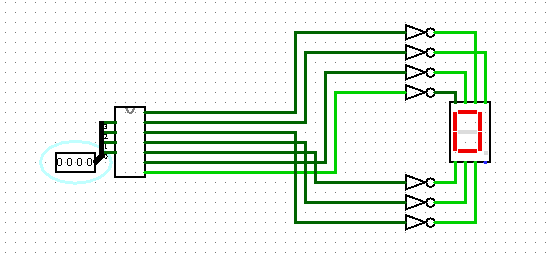
\includegraphics[width=\linewidth]{ScreenshotsTests/Comp 1/Comp 1_00009.png}
    \caption{Test 1 - (binarnie) 0000, (dziesiętnie) 0}
    \label{fig:test0}
\end{figure}

Test 1 zakończony pomyślnie.

\begin{figure}[H]
    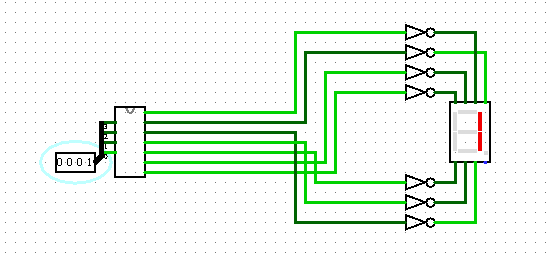
\includegraphics[width=\linewidth]{ScreenshotsTests/Comp 1/Comp 1_00008.png}
    \caption{Test 2 - (binarnie) 0001, (dziesiętnie) 1}
    \label{fig:test1}
\end{figure}

Test 2 zakończony pomyślnie.

\begin{figure}[H]
    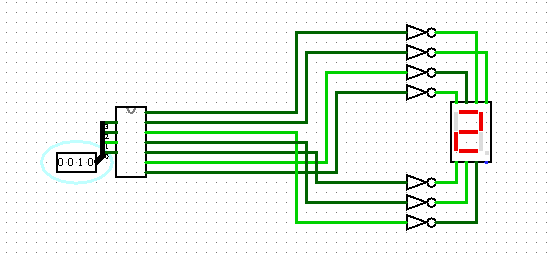
\includegraphics[width=\linewidth]{ScreenshotsTests/Comp 1/Comp 1_00007.png}
    \caption{Test 3 - (binarnie) 0010, (dziesiętnie) 2}
    \label{fig:test2}
\end{figure}

Test 3 zakończony pomyślnie.

\begin{figure}[H]
    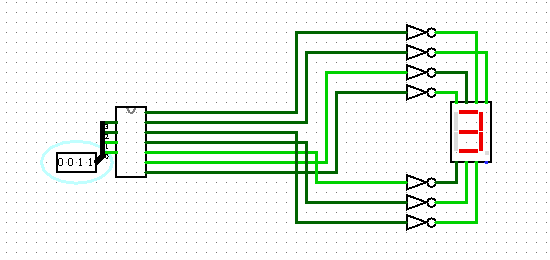
\includegraphics[width=\linewidth]{ScreenshotsTests/Comp 1/Comp 1_00006.png}
    \caption{Test 4 - (binarnie) 0011, (dziesiętnie) 3}
    \label{fig:test3}
\end{figure}

Test 4 zakończony pomyślnie.

\begin{figure}[H]
    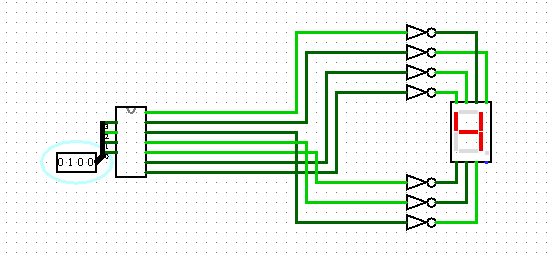
\includegraphics[width=\linewidth]{ScreenshotsTests/Comp 1/Comp 1_00005.png}
    \caption{Test 5 - (binarnie) 0100, (dziesiętnie) 4}
    \label{fig:test4}
\end{figure}

Test 5 zakończony pomyślnie.

\begin{figure}[H]
    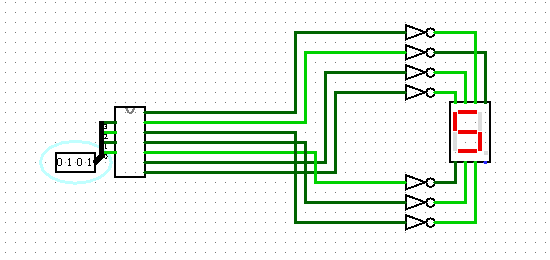
\includegraphics[width=\linewidth]{ScreenshotsTests/Comp 1/Comp 1_00004.png}
    \caption{Test 6 - (binarnie) 0101, (dziesiętnie) 5}
    \label{fig:test5}
\end{figure}

Test 6 zakończony pomyślnie.

\begin{figure}[H]
    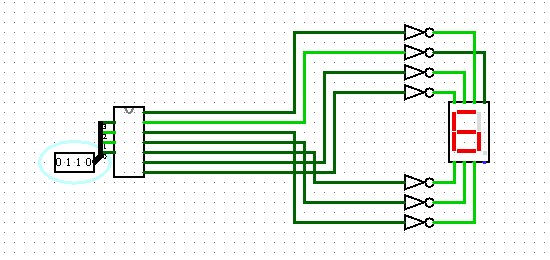
\includegraphics[width=\linewidth]{ScreenshotsTests/Comp 1/Comp 1_00003.png}
    \caption{Test 7 - (binarnie) 0110, (dziesiętnie) 6}
    \label{fig:test6}
\end{figure}

Test 7 zakończony pomyślnie.

\begin{figure}[H]
    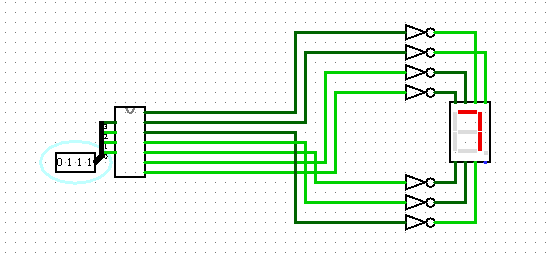
\includegraphics[width=\linewidth]{ScreenshotsTests/Comp 1/Comp 1_00002.png}
    \caption{Test 8 - (binarnie) 0111, (dziesiętnie) 7}
    \label{fig:test7}
\end{figure}

Test 8 zakończony pomyślnie.

\begin{figure}[H]
    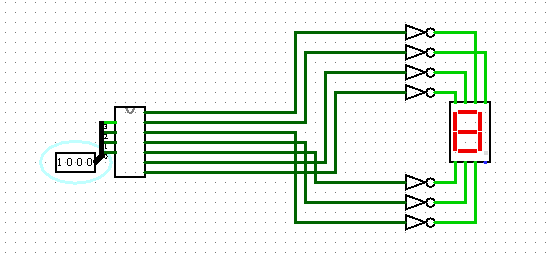
\includegraphics[width=\linewidth]{ScreenshotsTests/Comp 1/Comp 1_00001.png}
    \caption{Test 9 - (binarnie) 1000, (dziesiętnie) 8}
    \label{fig:test8}
\end{figure}

Test 9 zakończony pomyślnie.

\begin{figure}[H]
    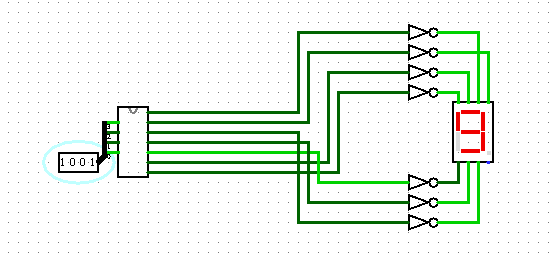
\includegraphics[width=\linewidth]{ScreenshotsTests/Comp 1/Comp 1_00000.png}
    \caption{Test 10 - (binarnie) 1001, (dziesiętnie) 9}
    \label{fig:test9}
\end{figure}

Test 10 zakończony pomyślnie.

\subsection{Ocena}\label{subsec:qa-review}
Moduł 7digit.circ spełnia założenia QA.

\end{document}